\chapter{外骨骼数据采集与步态分析系统}

外骨骼是一个融合各种传感器的智能系统,可靠的传感器数据才能保证控制算法的性能。本章针对研究的踝关节式外骨骼搭建了一套传感器系统,包括以dSPACE为核心的处理器、测量外骨骼力矩的应变电桥、测量步态周期的足底开关、惯性测量单元IMU、表面肌电信号sEMG等,如图2.1所示。

\begin{figure}[htb]
    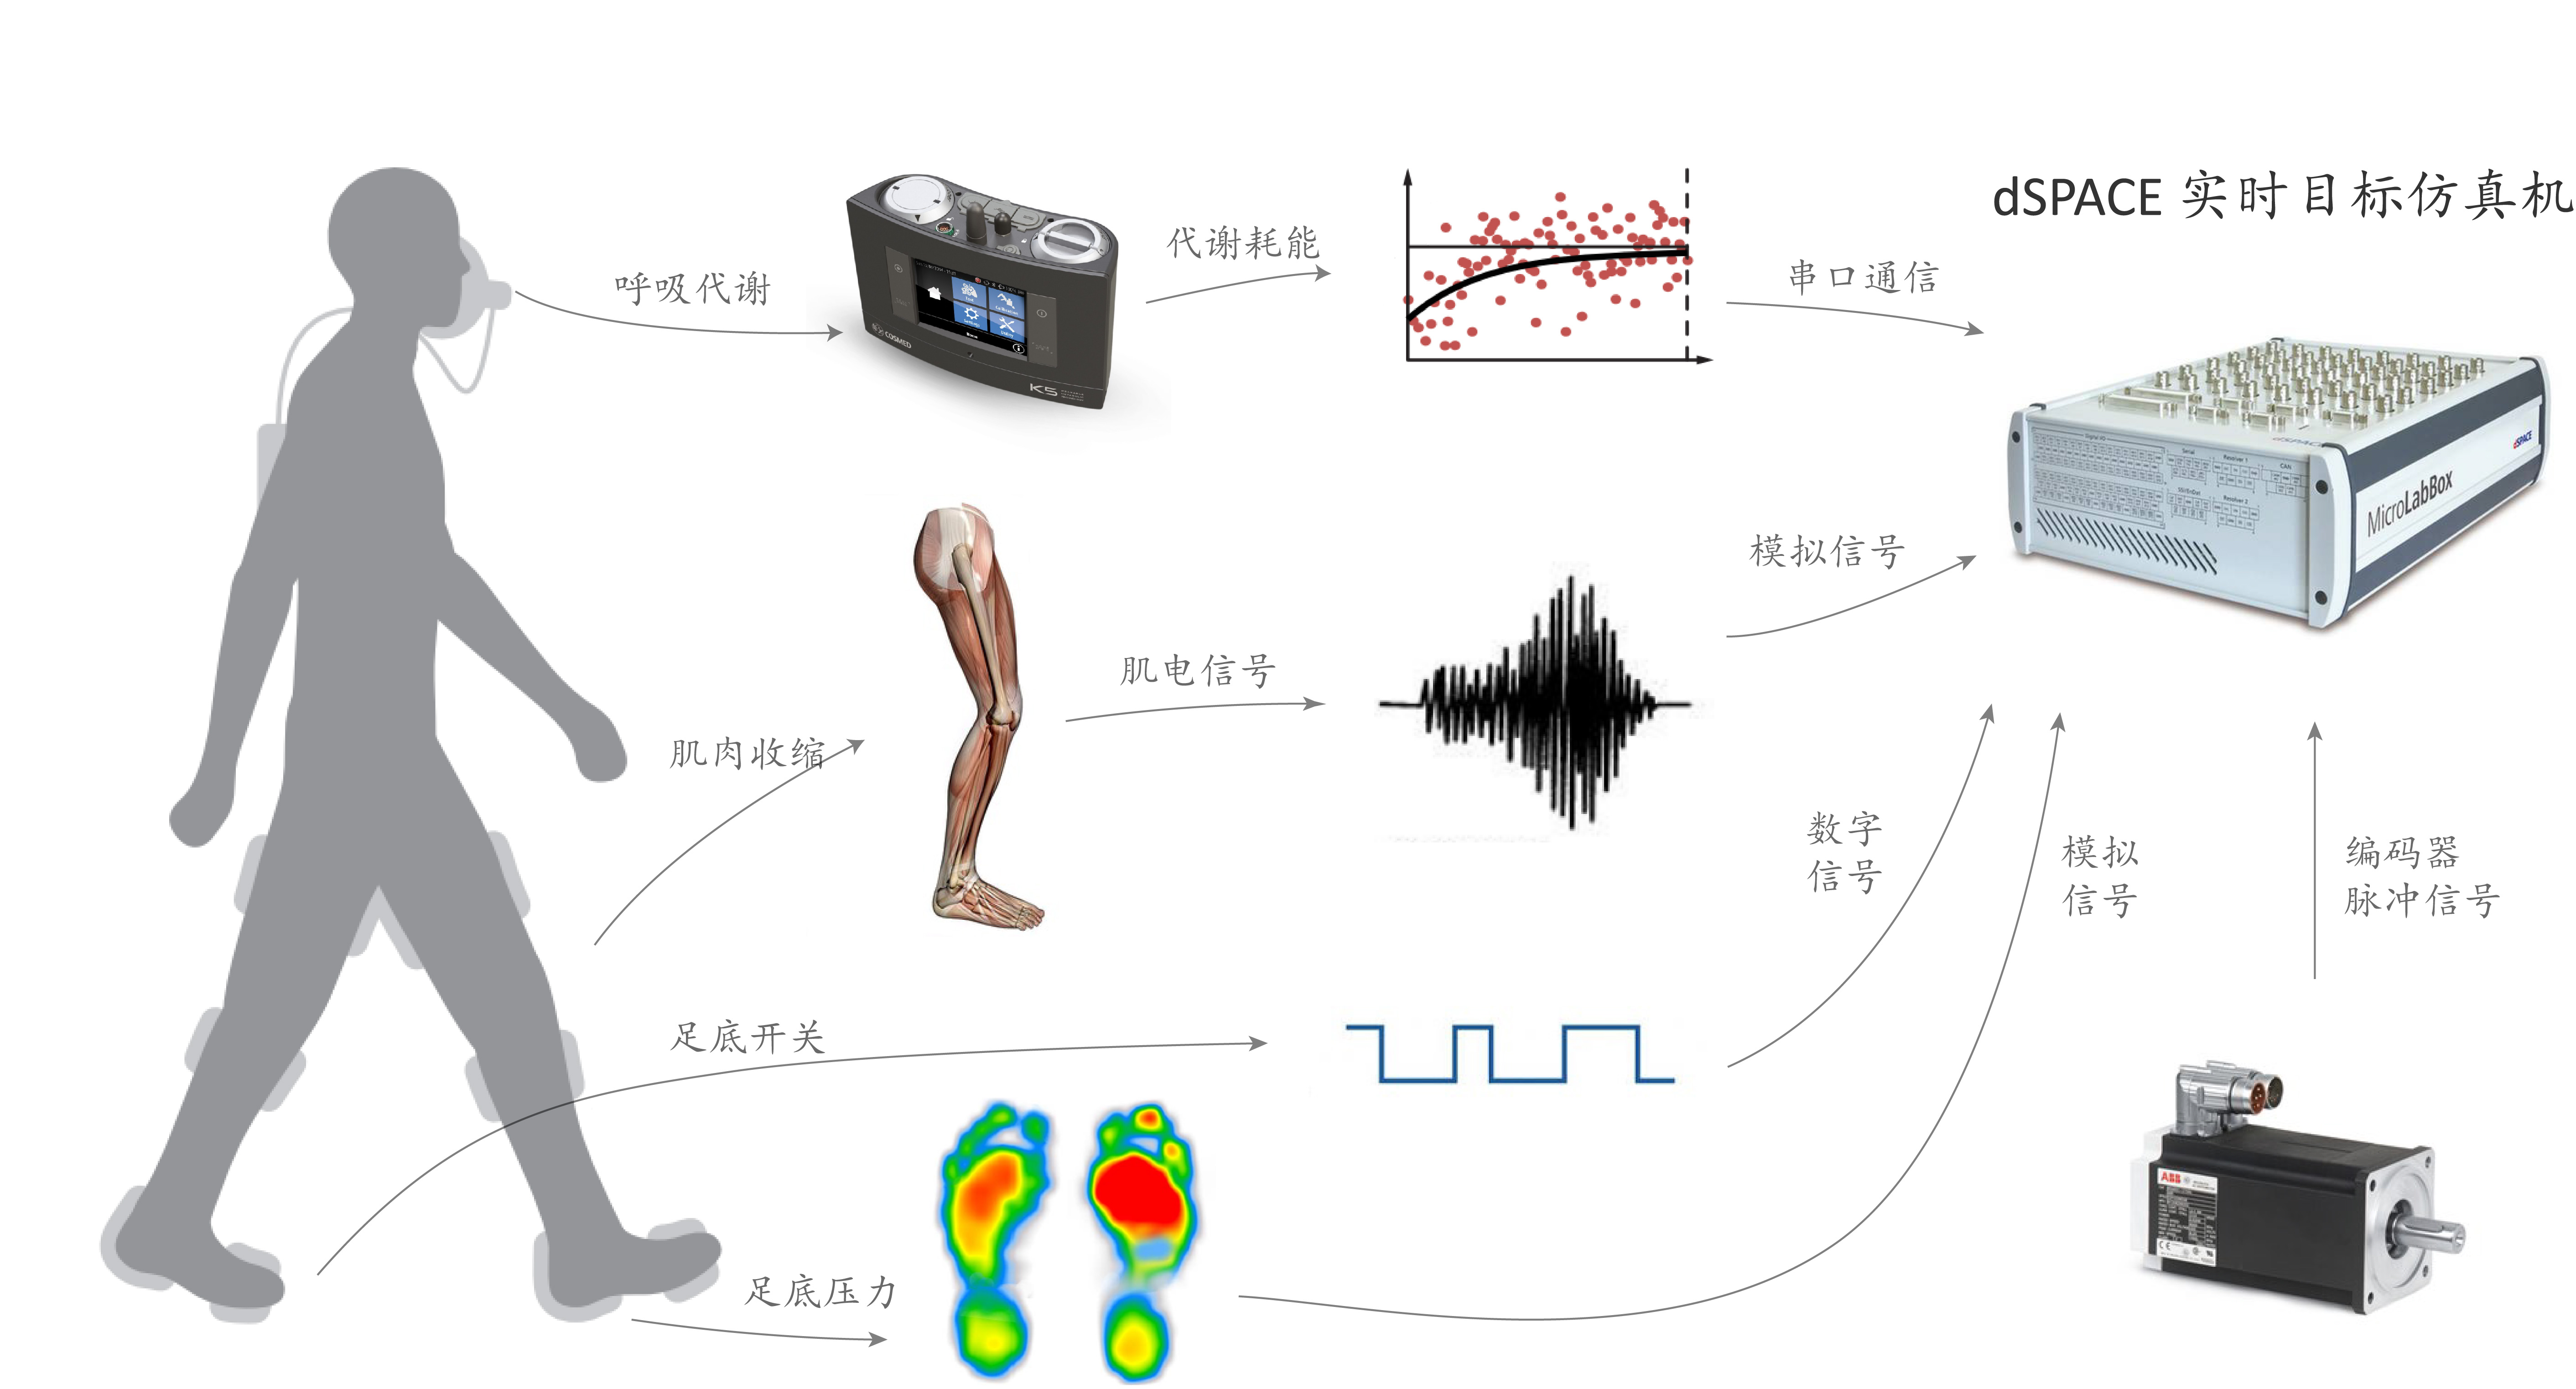
\includegraphics[width=15cm]{fig/f27.jpg}
    \caption{踝关节外骨骼的数据采集系统}
    \label{fig:mark}
\end{figure}

\section{dSPACE实时目标机MicroLabBox}

实时目标机是由德斯拜斯(dSPACE)公司开发的一套基于MATLAB/Simulink的控制系统开发及半实物仿真软硬件工作平台,它可以方便的与Matlab/Simulink进行连接,实现快速控制原型(RCP)或硬件在环仿真(HIL)。dSPACE通过Simulink进行控制算法的快速开发、代码生成与测试调试,具有强实时性、可靠性高、扩充性好的特点,目前已广泛应用于汽车、机器人、航空航天等领域。

\subsection{dSPACE的硬件平台}

\begin{figure}[htb]
    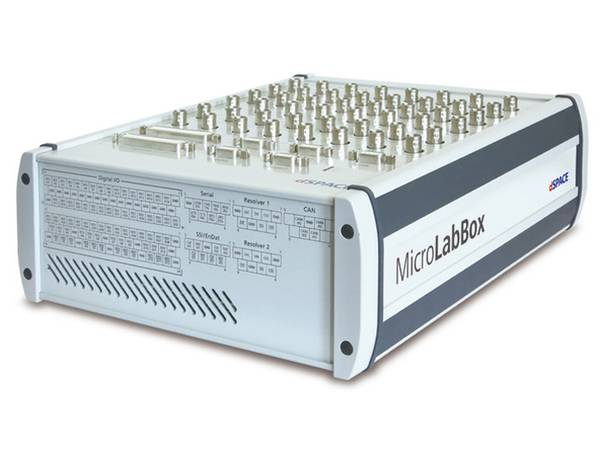
\includegraphics[width=8cm]{fig/f21.jpeg}
    \caption{dSPACE的实时目标机MicroLabBox}
    \label{fig:mark}
\end{figure}

MicroLabBox是dSPACE面向实验室推出的一款紧凑型实时仿真平台,如图2.1所示,具有高速的计算能力和快速的输入输出特性。CPU采用2GHz双核实时处理器(Freescale Power QorIQ 5020),最快可以实现15us的闭环控制周期,同时还可以使用内部集成的FPGA加速并行计算。MicroLabBox同时具有丰富的外设,48通道数字I/O接口、32通道模拟量输入接口、16通道模拟量输出接口,同时配有2个CAN总线收发器、1个RS-232串口、一个网络接口、6通道正交编码器接口等。除此之外,MicroLabBox中集成的稳压电源可以为传感器进行供电,使系统使用起来更加方便。

\subsection{dSPACE的软件平台}
(1)实时接口RTI

MicroLabBox与Simulink的连接是通过实时接口RTI来实现的。它可以看做是Simulink下关于MicroLabBox的一些模块,通过这些模块可以实现对MicroLabBox各种I/O接口的配置与初始化,并可以与Simulink中的其他模块,如控制模块、滤波模块相连接,从而实现数据采集与处理和控制系统的搭建。模型搭建完毕后,可以通过调用MATLAB的RTW工具对模型进行编译,自动生成适用于MicroLabBox的目标代码,并下载到MicroLabBox中完成Simulink模型预期实现的功能。
    
(2)ControlDesk

ControlDesk是dSAPCE公司开发的一种图形化的人机交互软件,能够提供虚拟示波器、虚拟按钮、虚拟表盘等功能,如图2.2所示。根据ControlDesk提供的各种工具,用户可以快速设计出适合项目的可视化界面,方便的对程序中的变量进行监控、修改参数、记录数据。

\begin{figure}[htb]
    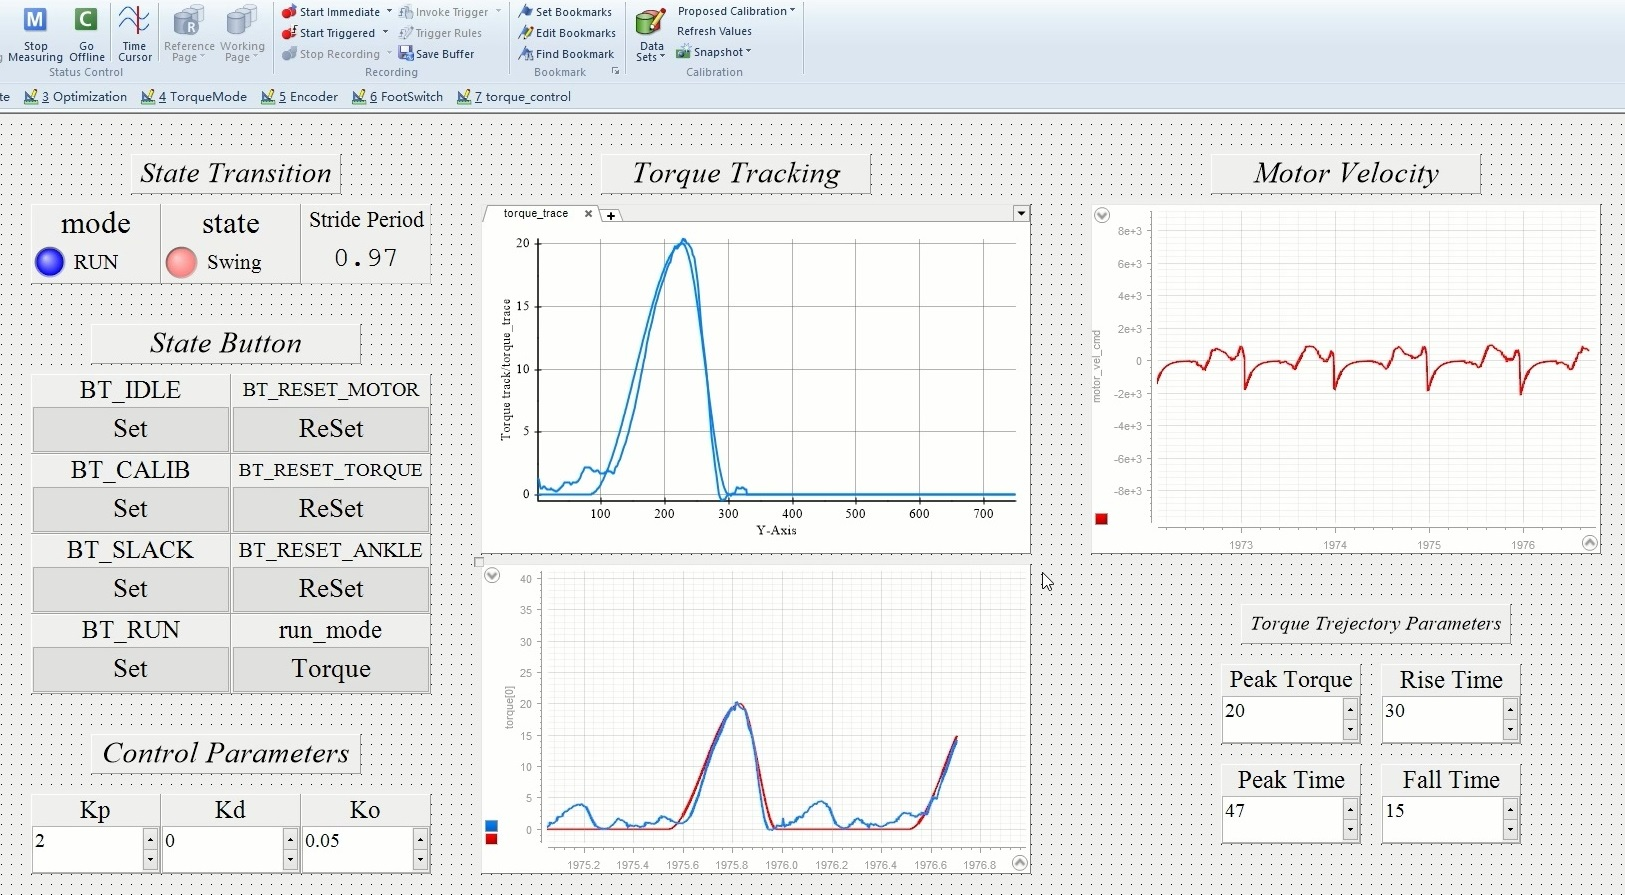
\includegraphics[width=14cm]{fig/f22.jpg}
    \caption{dSPACE的实时目标机MicroLabBox}
    \label{fig:mark}
\end{figure}

由于MicroLabBox可以借助Simulink以模块化的方式进行开发,并可以利用ControlDesk快速设计出对应的上位机界面,因此本文工作将以MicroLabBox为核心,进行数据采集、处理与外骨骼控制。

\section{外骨骼力矩测量}

\begin{figure}[htb]
    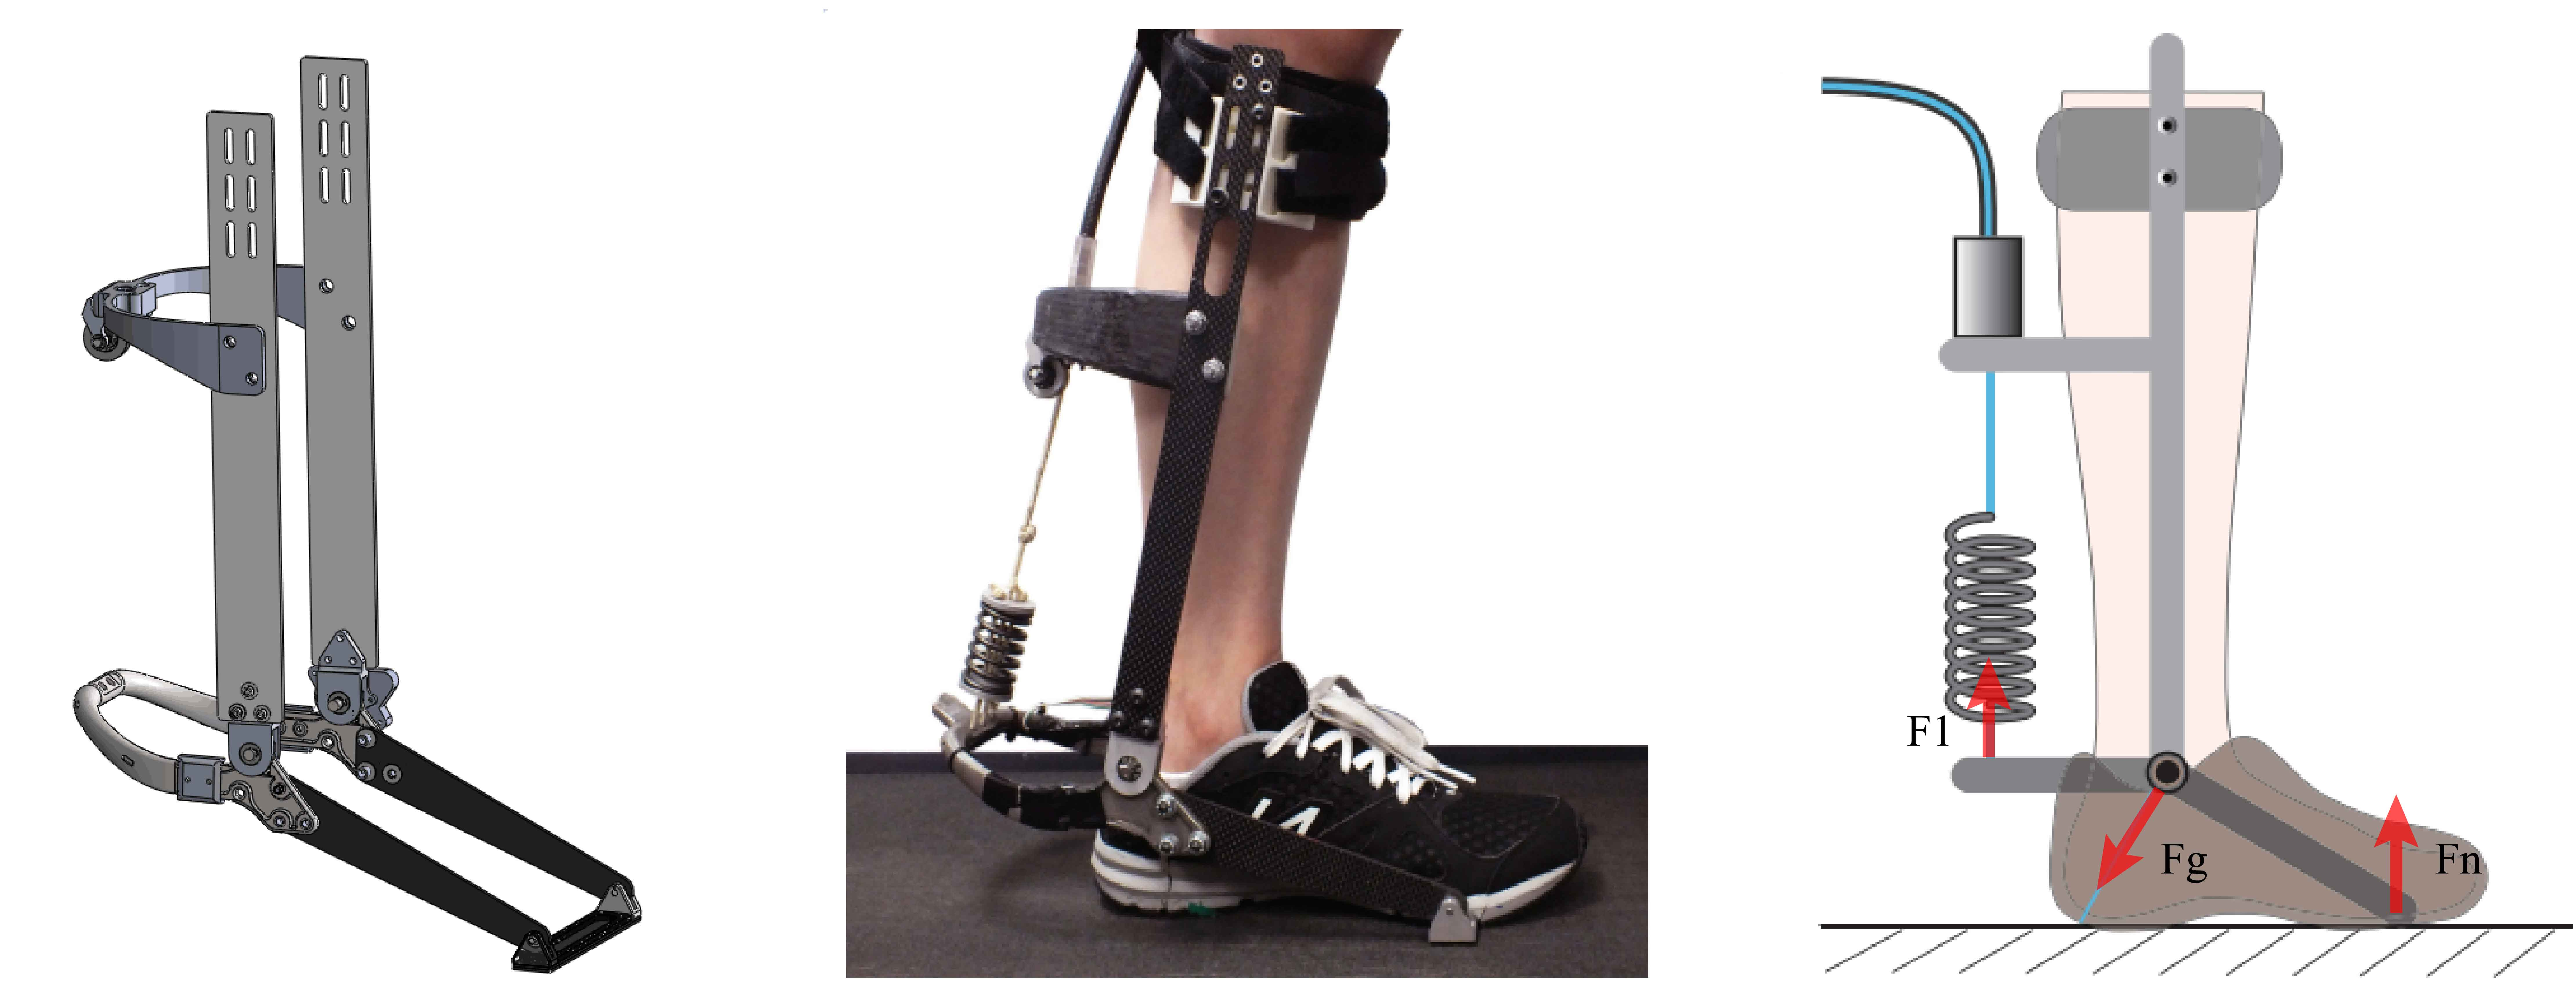
\includegraphics[width=14cm]{fig/f23.jpg}
    \caption{dSPACE的实时目标机MicroLabBox}
    \label{fig:mark}
\end{figure}

为了现实外骨骼的力矩控制,必须要对人机之间的交互力矩加以测量。外骨骼的结构与受力分布如图2.3所示。当电机通过鲍登线和SEA对外骨骼和穿戴者施加作用力$F1$时,由材料力学可知外骨骼的钛合金悬臂会在拉力的作用下发生变形,如图2.4 a)所示。通过应变片测量出钛合金悬臂的变形程度,即可得到电机施加的驱动力矩。

\begin{figure}[htb]
    \subfloat[外骨骼悬臂在拉力作用下发生变形]{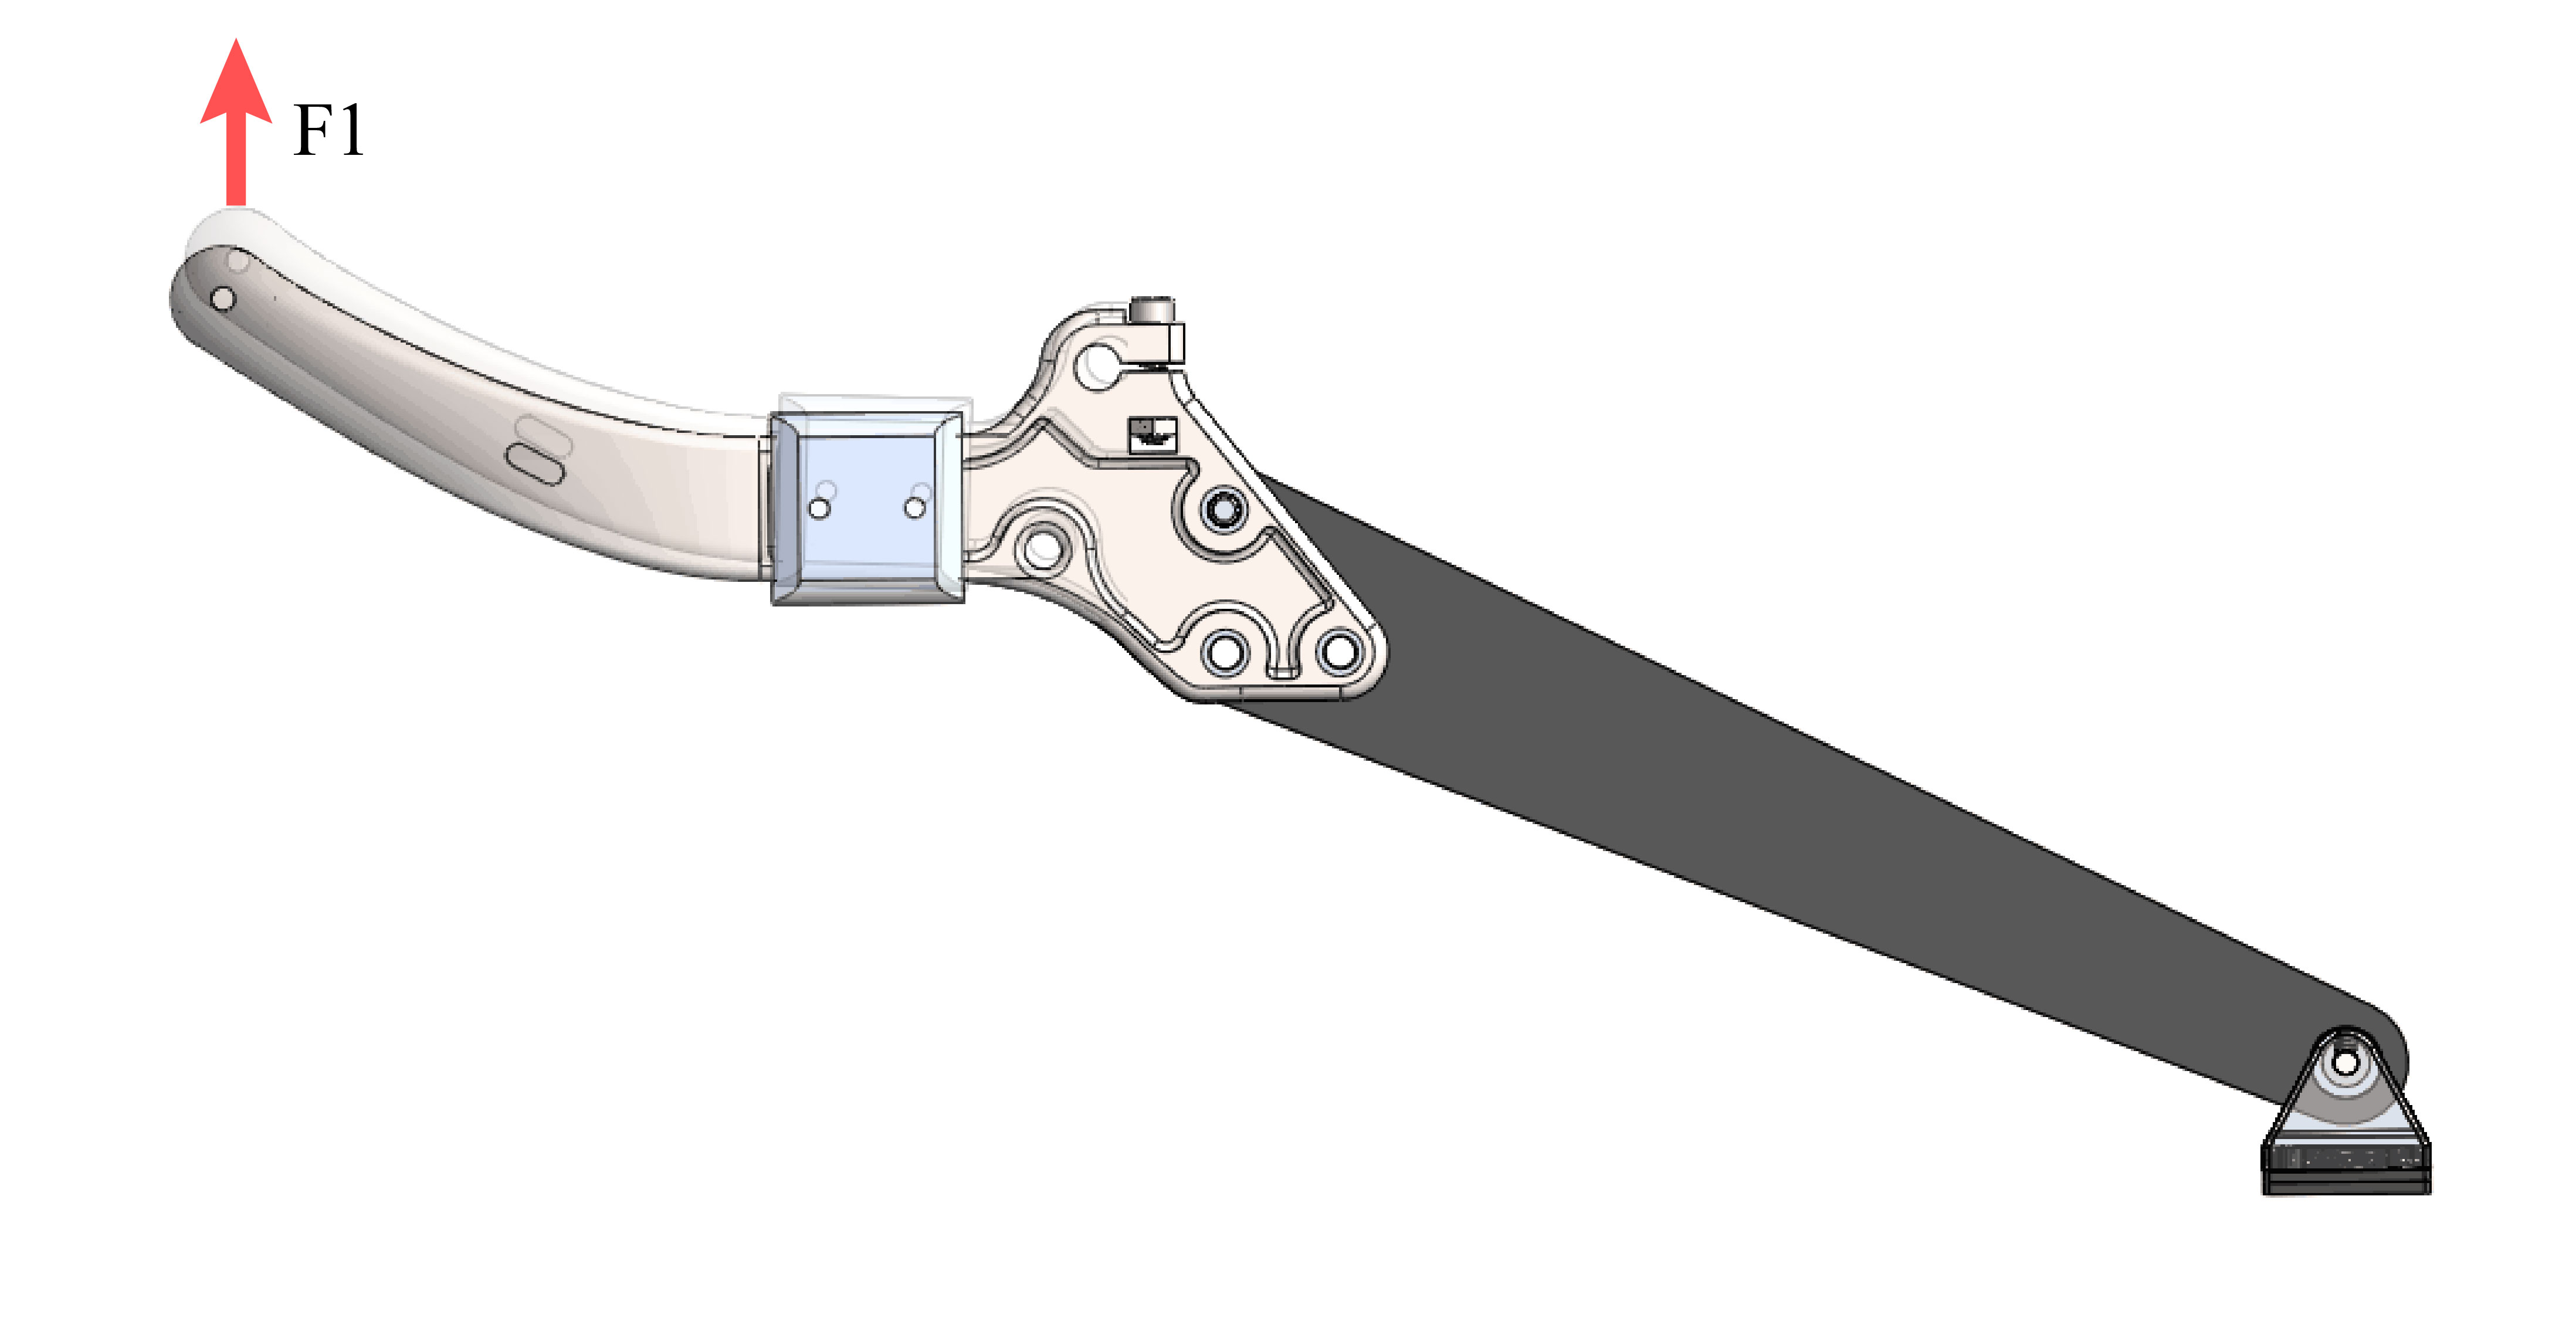
\includegraphics[width=7.5cm]{fig/f24.jpg}}\quad
    \subfloat[应变电桥的安装位置]{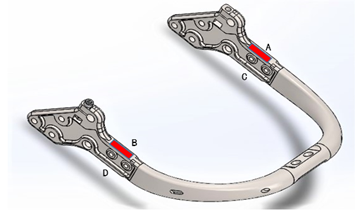
\includegraphics[width=6cm]{fig/f25.png}}
    \caption{外骨骼力矩测量原理}
    \label{fig:subfigss}
\end{figure}

\begin{figure}[htb]
    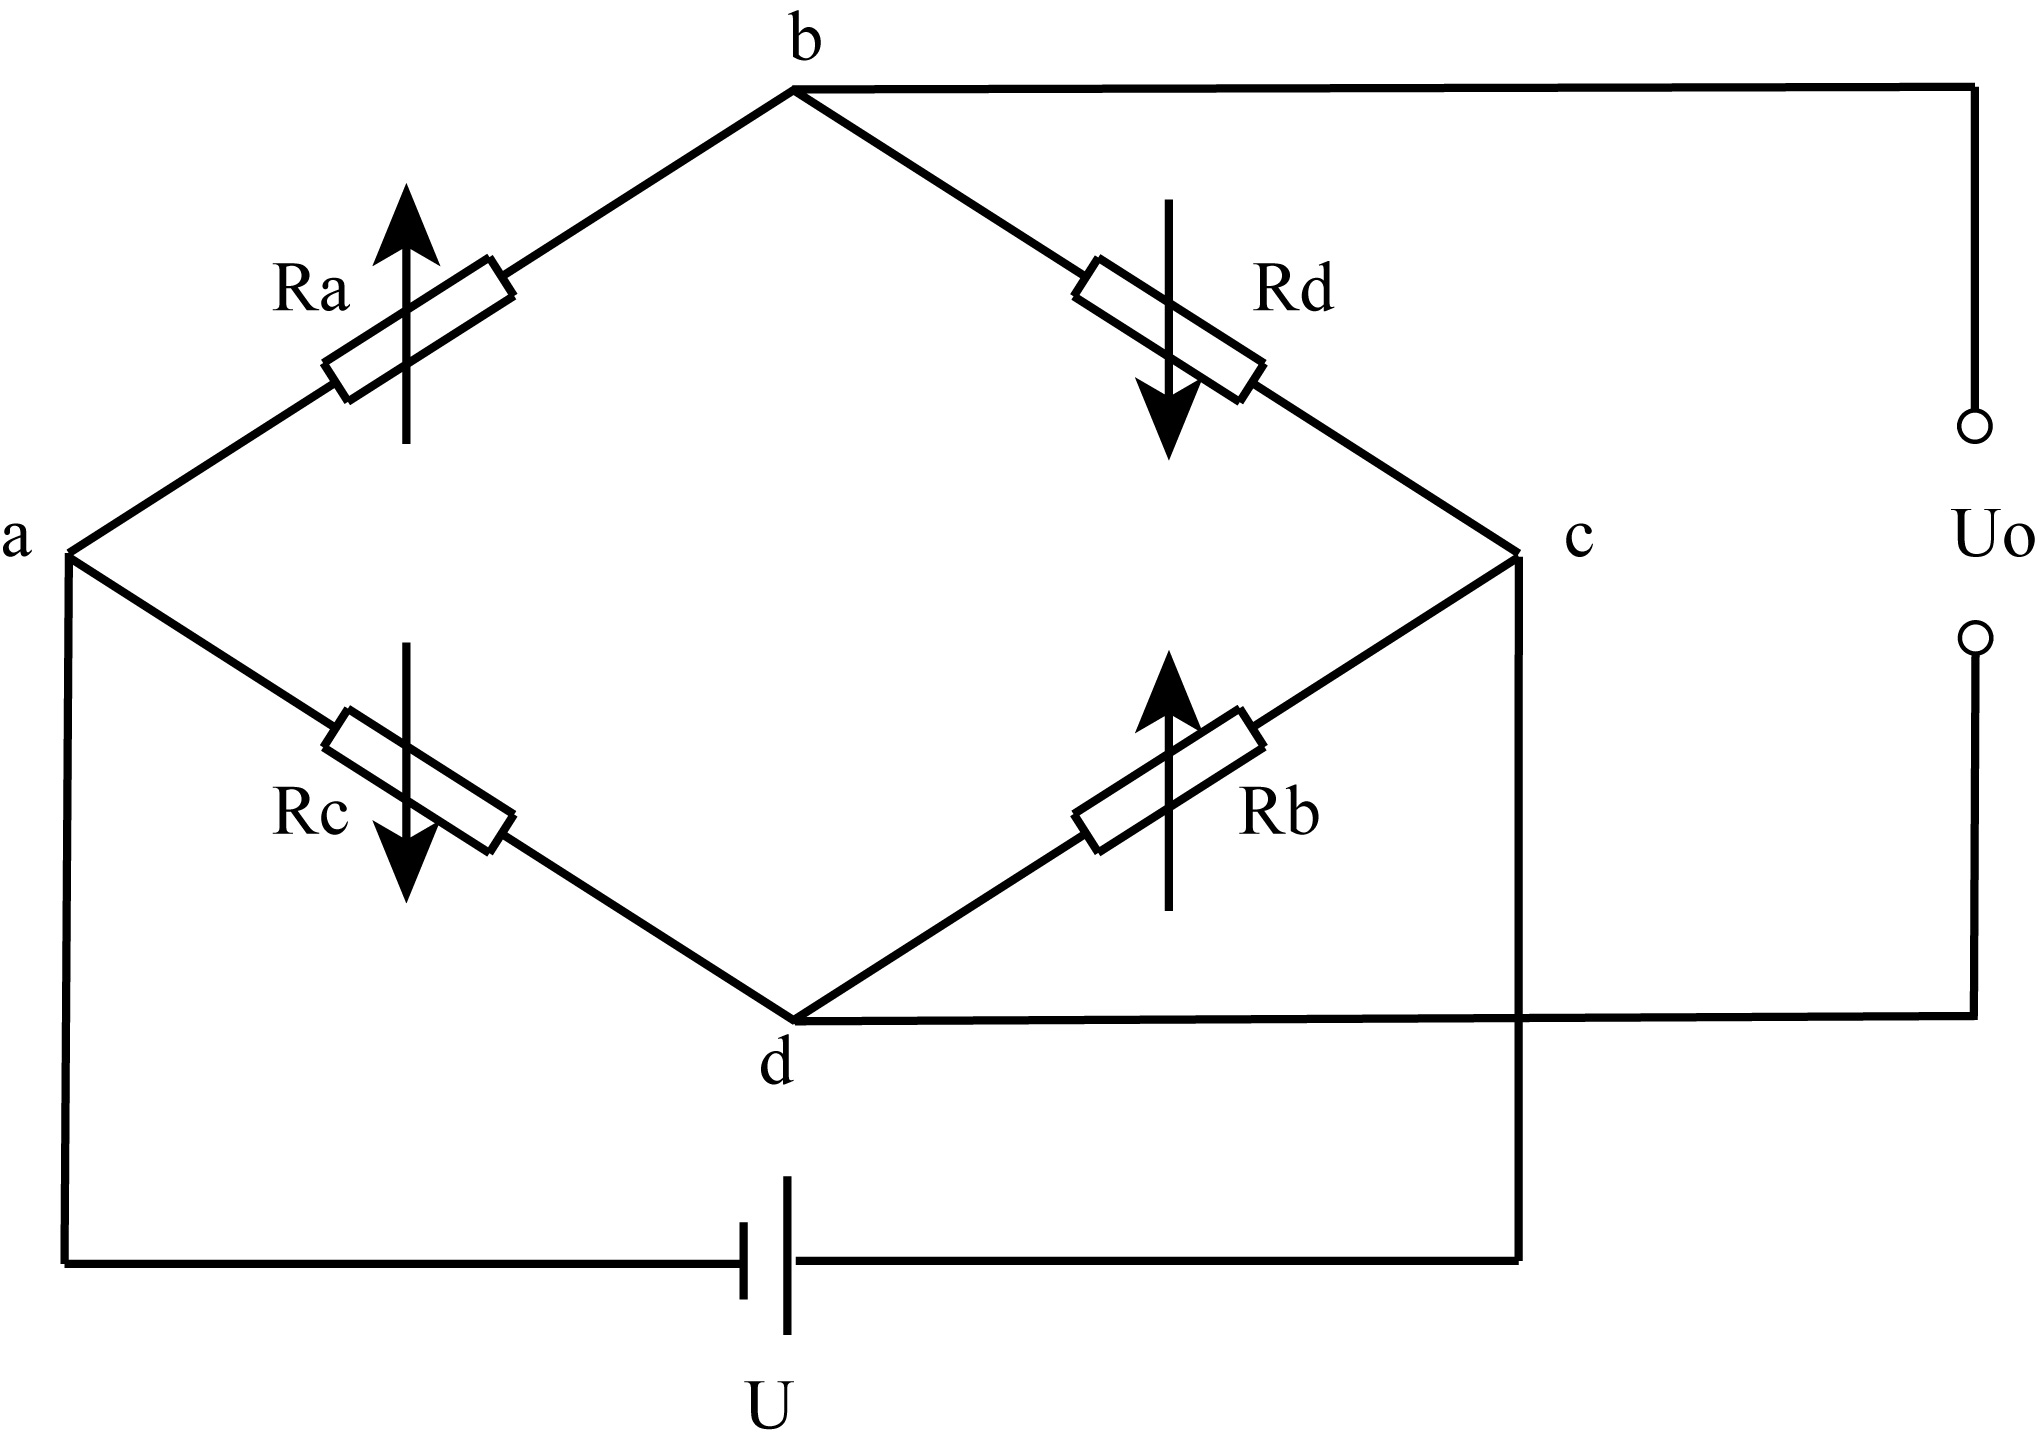
\includegraphics[width=8cm]{fig/f25.jpg}
    \caption{差动全桥应变测量电路}
    \label{fig:mark}
\end{figure}

这里使用差动全桥对应变进行测量,由如图2.5电路可得:
\begin{align}
U_o = U\cdot \frac{(R_a + \Delta R_a)(R_b + \Delta R_b) - (R_c - \Delta R_c)(R_d - \Delta R_d)}{(R_a + \Delta R_a + R_d - \Delta R_d)(R_b + \Delta R_b + R_c - \Delta R_c)}
\end{align}

设$R_a = R_b = R_c = R_d$,则:
\begin{align}
U_o = U\cdot \frac{\Delta R_a R_b + \Delta R_b R_a + \Delta R_c R_d + \Delta R_d R_c}{(R_a + R_d)(R_b + R_c)}= U\cdot \frac{\Delta R_a}{R_a}
\end{align}

选型上,项目中采用OMEGA公司的KFH-6-350-C1-11L1M2R的电阻应变片,使用FUTEK-IAA100放大器对全桥电路信号进行测量和放大,之后通过MicroLabBox的模拟量输入接口进行读取,并用于后续的力矩反馈控制。

\section{步态分析与步态周期测量}
\subsection{人体下肢运动步态分析}

为了能够对穿戴者提供有益的辅助作用,需要要对人体行走过程进行加以分析。步态周期是人体基本的运动之一,它定义为连续发生两次重复的步行事件之间的时间间隔。虽然可以选择任何事件来定义步态循环,但通常使用一只脚接触地面的瞬间(初始接触)作为开始。如果决定从右脚的初始着地开始,则到右脚再次接触地面为止,并如此循环。

\begin{figure}[htb]
    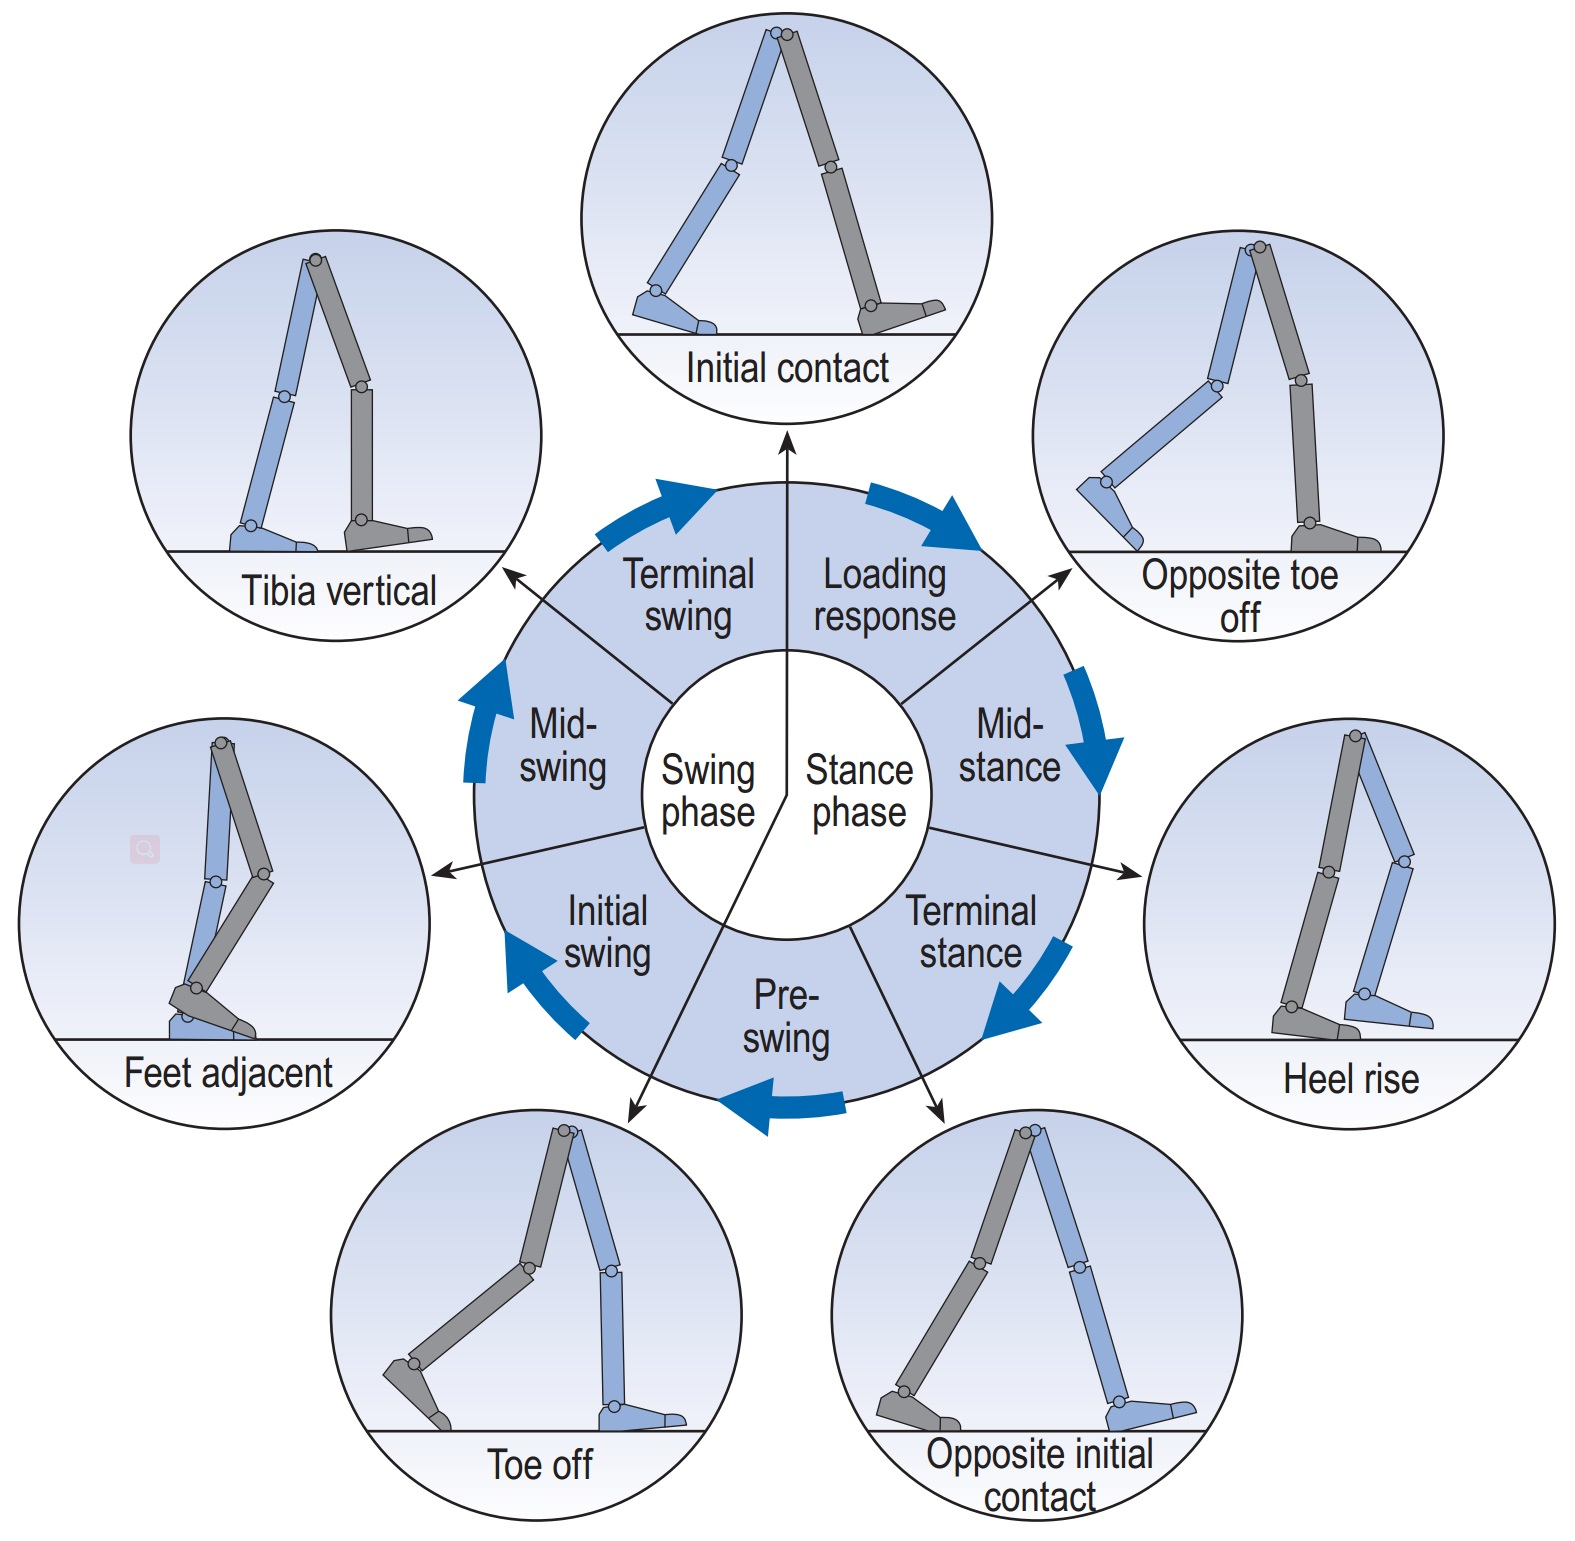
\includegraphics[width=14cm]{fig/f29.jpg}
    \caption{步态周期经历的过程}
    \label{fig:mark}
\end{figure}

如图2.7所示,在步态分析的教材\cite{p44}中,一般以7个术语件来定义步态周期的主要事件:
\begin{enumerate}
    \item 初始着地(Initial contact, IC)
    \item 反向脚趾离地(Opposite toe off, OT)
    \item 脚跟抬起(Heel rise, HR)
    \item 反侧初始着地(Opposite initial contact, OI)
    \item 脚趾离地(Toe off, TO)
    \item 双脚靠近(Feet adjacent, FA)
    \item 胫骨垂直(Tibia vertical, TV)
\end{enumerate}

这七个事件将步态循环分为7个阶段,其中4个阶段发生在脚着地时的站立相,3个阶段发生在脚在空中向前移动时的摆动相。站立相从初始着地一直持续到脚趾离地,并分为以下四个部分:
\begin{enumerate}
    \item 支撑初期(Loading response)
    \item 支撑中期(Mid-stance)
    \item 支撑末期(Terminal stance)
    \item 预摆动(Pre-swing)
\end{enumerate}

摆动相从脚趾离地开始持续到到下一次的初始着地。它又细分为:
\begin{enumerate}
    \item 摆动初期(Initial swing)
    \item 摆动中期(Mid-swing)
    \item 摆动末期(Terminal swing)
\end{enumerate}

\begin{figure}[htb]
    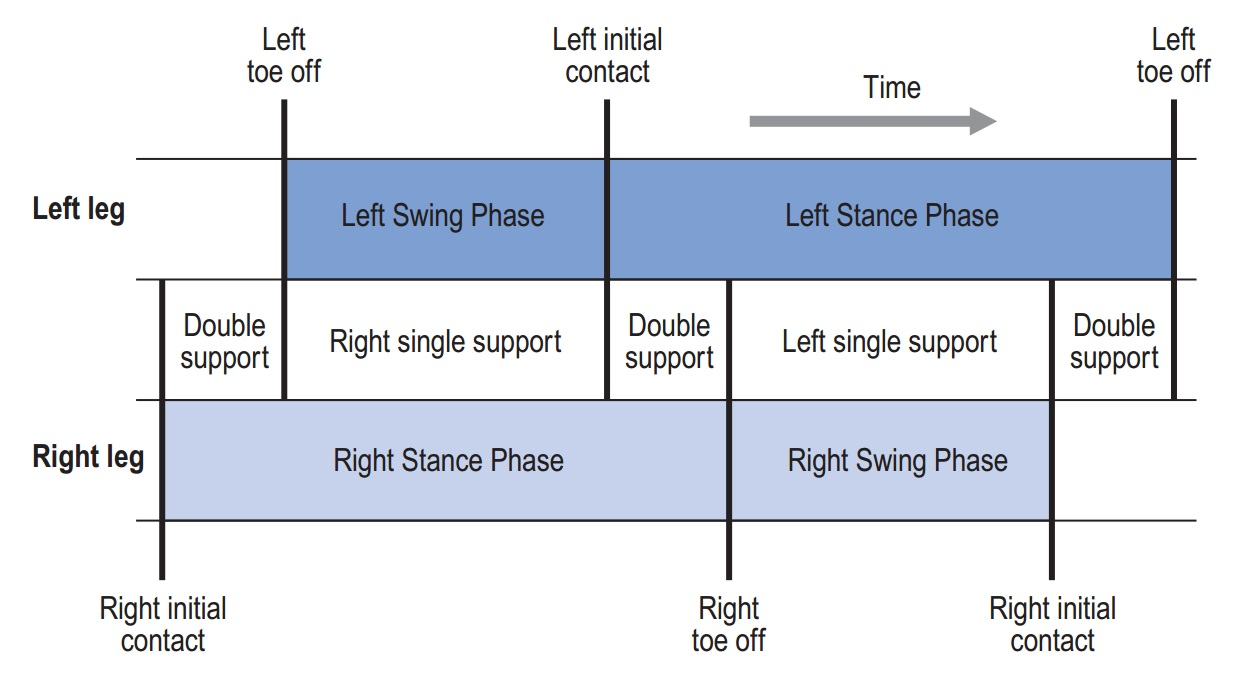
\includegraphics[width=15cm]{fig/f30.jpg}
    \caption{步态周期的时序}
    \label{fig:mark}
\end{figure}

图2.8显示了在一个多步态周期内,两只脚初始着地和脚趾离地的时间。当左脚还在地面上时,右脚开始接触地面,在右脚开始接触和左脚脚趾离开之间有一段时间的双支撑。在左腿摆动期间,只有右脚着地,右脚单支撑一段时间,并以左脚初始着地地面结束。然后是另一段双支撑期,直到右脚脚趾离地。左脚单支撑对应于右摆动相,周期结束时,下一个初始着地点在右侧。

因此,在每个步态周期中,有两个双支撑周期和两个单支撑周期。支撑相通常持续约60\%的周期,摆动相约40\%,每一阶段的双支撑约10\%。然而,这是随着行走速度的增加而变化的,随着速度的增加,摆动相成比例地变长,站立相和双支撑变短。双支撑阶段的消失也标志着从步行转变为跑步。

\subsection{基于足底开关的步态周期测量}

本文第三章在进行外骨骼力矩控制时,施加的力矩曲线与步态周期百分比具有密切关系。为了做到外骨骼控制与人体运动的同步,必须对步态周期进行准确的测量。常用的有使用足底开关、足底压力、关节角度等方法,本文采用简单且可靠的足底开关。

\begin{figure}[htb]
    \subfloat[足底开关]{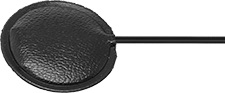
\includegraphics[width=6cm]{fig/f31.jpg}}\quad
    \subfloat[步态检测状态机]{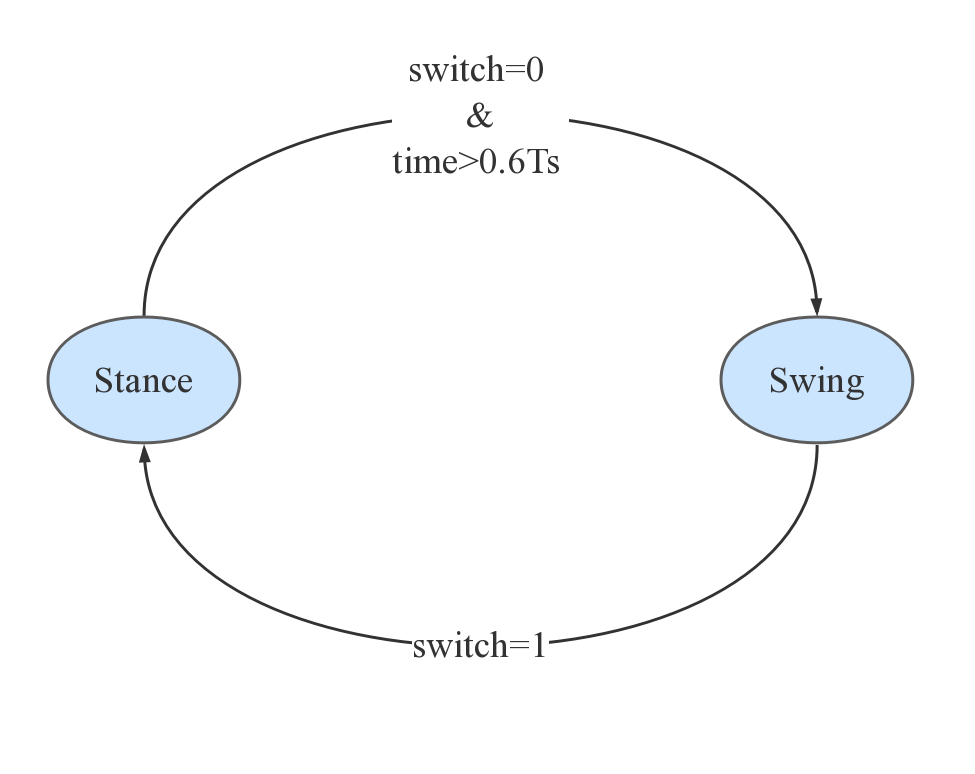
\includegraphics[width=8cm]{fig/f32.jpg}}
    \caption{足底开关与步态检测状态机}
    \label{fig:subfigss}
\end{figure}

如图2.9 a)所示的薄膜式接触开关被粘贴在外骨骼鞋子内部脚跟处,用以测量步态周期。传感器的两端连接到MicroLabBox的数字引脚上,一端配置为高电平的数字输出,另一端配置为下拉状态的数字输入。当足底开关所在腿处于摆动阶段时,开关处于断开状态,输入信号为低电平;当其切换到支撑阶段时,开关连通使输入信号变为高电平。由此可以对摆动相和支撑相进行检测,每次摆动相切换到支撑相时,便进入到一个新的步态循环,两个上升沿之间的时间便为一个步态周期的时间。

在实验中使用足底开关进行测量时会出现毛刺现象,因此单纯通过采集信号的高低电平来判断相位变化不甚可靠。为此本文提出一种步态检测状态机,如图2.9 b)所示,摆动相转换支撑相时,只通过高电平判断,这样可以准确测量到步态周期的开始时刻。在支撑相转换到摆动相时,除了电平还要做一个时间检测,只有在当前步的时间大于前一步完整步态周期时间的60\%时,才由支撑相转换到摆动相。通过此方法可以准确检测摆动-支撑的转换,同时可以有效的消除信号毛刺,但无法检测出支撑-摆动的转换,此转换根据人体步态过程的统计规律得到。

\begin{figure}[htb]
    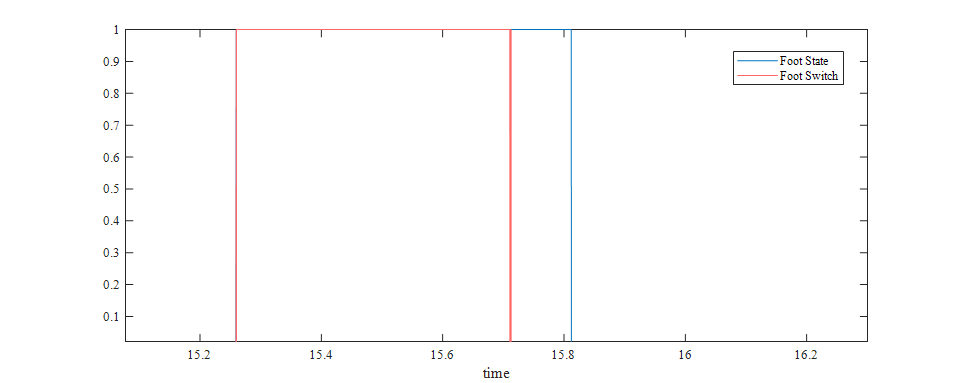
\includegraphics[width=16cm]{fig/f33.png}
    \caption{足底开关信号与步态检测}
    \label{fig:mark}
\end{figure}

\section{IMU原理}
\subsection{IMU原理与Kalman滤波}
IMU即惯性测量单元,它可以测量得到物体的加速度和角速度信息。IMU可以根据自由度(DoF)的不同分为不同的类型,6DoF的IMU中包含三轴加速度计和三轴陀螺仪。三轴加速度计能够测量三个方向上加速度的大小,三轴陀螺仪能够测量三个轴角速度的大小,如图中2.11(a)所示。

\begin{figure}[htb]
    \subfloat[IMU]{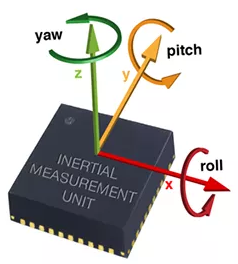
\includegraphics[width=3.5cm]{fig/f34.png}}
    \subfloat[加速度计]{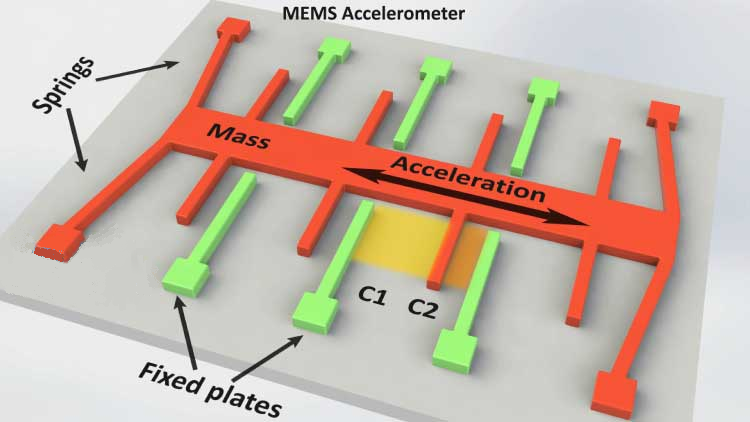
\includegraphics[width=6.5cm]{fig/f35.png}}
    \subfloat[陀螺仪]{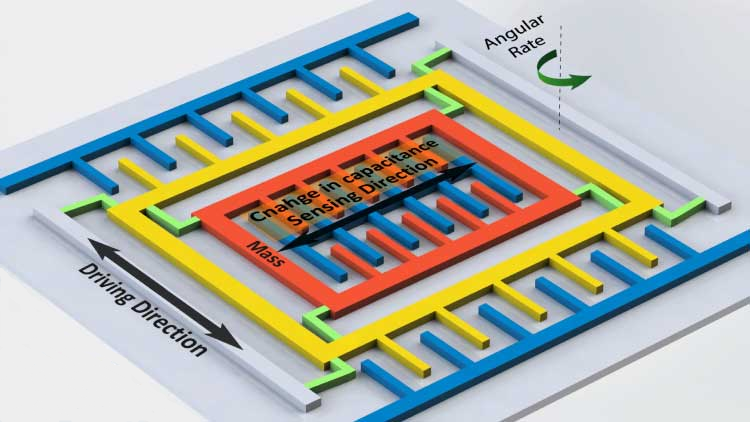
\includegraphics[width=6.5cm]{fig/f36.png}}
    \caption{IMU与其内部构成}
    \label{fig:subfigss}
\end{figure}

加速度的测量利用了牛顿第二定律。如图2.11(b)所示,中间红色的为一个质量块,两头通过具有弹簧性质的杆状结构与基底相连,红色的短栅与绿色的短栅分别为电容的极板。当传感器在箭头方向受到加速度$a$时,由于质量块与基底相连因而有相同的加速度,这个加速度的由弹簧产生,根据$f=ma=kx$,质量块会沿加速度相反的方向移动一定距离,即红色极板与绿色极板之间的距离会发生变化。通过测量极板电容C的变化就可以得到加速度的大小。在三轴加速度计中,这样的结构在三个方向各有一个,且做到了微米的尺寸,并配合相应的测量电路集成在一个芯片中,构成一个微机电系统(MEMS)。

角速度测量的原理比加速度要复杂一些,它利用了科里奥里力(Coriolis Force)。当物体在旋转的坐标系下运动时,由于坐标系的旋转会在垂直其运动方向上受到一个作用力,即科里奥里力,$F=-2mvω$。科里奥里力是由坐标系的转动与物体在动坐标系中的相对运动引起的,其本质是物体的惯性。

陀螺仪的物理实现如图2.11 c)所示,外侧的蓝色与黄色部分为驱动电极,内部的红色与蓝色为测量电极。首先在模块的驱动方向施加正弦驱动电压,使模块沿驱动方向做正弦运动。当模块发生旋转时,质量块受科里奥里力影响在测量方向会发生运动,而且是正弦运动,且正弦运动的幅值与角速度成正比,通过电极测量出此幅值,便可以得到模块角速度。与三轴加速度计一样,这样的结构在三轴陀螺仪的三个方向上各有一个,从而测量出三个方向的角速度。

\subsection{IMU姿态解算与数据融合}

\begin{figure}[htb]
    \subfloat[IMU水平放置]{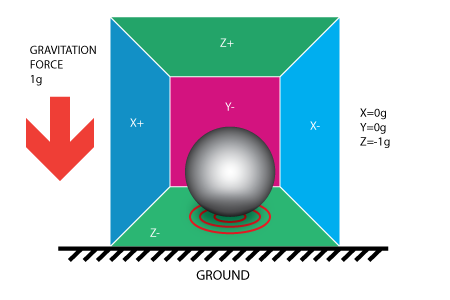
\includegraphics[width=8cm]{fig/f37.png}}\quad
    \subfloat[IMU倾斜放置]{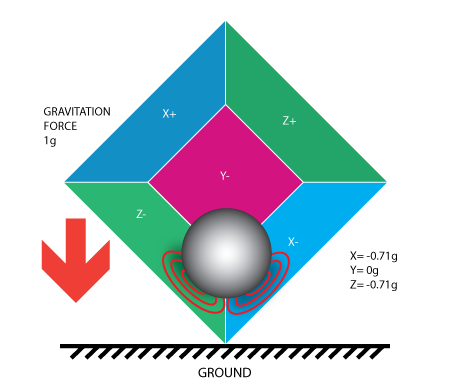
\includegraphics[width=7cm]{fig/f38.png}}
    \caption{通过加速度计解算角度信息}
    \label{fig:subfigss}
\end{figure}

加速度计和陀螺仪都无法直接得到角度数据,需要从加速度和角速度解算出角度信息。可以把加速度计中的质量块当做左图中的小球,由加速度计的原理可知,在传感器静止的时候,测量的结果为重力加速度,因此当传感器倾斜时,如右图所示,可以根据重力加速的在三轴分量的大小来解算出角度:
\begin{align}
Angle_{Accel} = arccos\frac{ax}{-g}
\end{align}
从角速度解算出角度更简单,只需要知道初始角度然后对角速度进行积分就可以了:
\begin{align}
Angle_{Gyro}=Angle_0 + \int_0^t Gyro dt
\end{align}
本文分析的仅为单轴的情况,对于三轴角度解算还需要涉及坐标系转换。

通过加速度和角速度都可以解算出角度信息,但这两种方式都存在很大的问题。加速度计由于容易受到振动的影响,噪声很大,所以解算出角度的噪声也很大;通过角速度积分得到角度的方式,由于初始角度并不能准确得到,而且角速度存在零偏和零漂问题,偏移误差会被累积导致角度不断漂移。因此,两种方式解算出来的角度都无法直接使用。

接下来采用Kalman滤波的方法,把两个传感器的数据融合在一起,得到一个既没有累计误差、噪声又小的角度信息。首先建立Kalman滤波器的状态观测方程。本文选择需要观测的角度$\theta$和陀螺仪角速度偏置$\omega_b$作为状态变量,陀螺仪的角速度为控制变量,加速度计解算得到的角度$\theta_{accel}$作为观测变量,并由此得到状态空间方程:

\begin{align}
\begin{bmatrix} \theta(k+1)  \\ \omega_b(k+1)   \end{bmatrix} &= \begin{bmatrix} 1 & -dt \\ 0 & 1   \end{bmatrix}\begin{bmatrix} \theta(k)  \\ \omega_b(k) \end{bmatrix} + \begin{bmatrix} dt \\ 0  \end{bmatrix} \omega(k) \\
\theta_{accel}(k) &=\begin{bmatrix} 1 & 0  \end{bmatrix}  \begin{bmatrix} \theta(k) \\ \omega_b(k)  \end{bmatrix}
\end{align}
其中式2.5为公式2.4的推广,式2.6中的$\theta_{accel}$由式2.3计算得到。之后令:
\begin{align}
X(k) = \begin{bmatrix} \theta(k)  \\ \omega_{b}(k) \\  \end{bmatrix}, \quad U(k) = \omega(k), \quad Y(k) = \theta_{accel}(k)
\end{align}
并将状态空间方程表示成如下标准形式:
\begin{align}
X(k+1) &= A X(k) + B U(k) + G W(k) \\
Y(k) &= C X(k) + V(k)
\end{align}

式中$W(k)$为输入白噪声,反应系统建模的不准确性;而$V(k)$表示观测噪声,反应传感器信号采集时的干扰噪声。

对于上面建立的状态空间方程,使用卡尔曼滤波器进行滤波。Kalman滤波方程组由五个方程组成:
\begin{align}
    状态一步预测: & \hat{X}(k+1|k) = A \hat{X}(k|k) + B U(k) \\
    状态更新:& \hat{X}(k+1|k+1) = A \hat{X}(k+1|k) + K(k+1)[Y(k+1)-C\hat{X}(k+1|k)] \\
    增益矩阵更新:& K(k+1) = P(k+1|k)C^T[CP(k+1|k)C^T + R]^{-1} \\
    协方差矩阵一步预测:& P(k+1|k) = AP(k|k)A^T+GQG^T \\
    协方更新:& P(k+1|k+1) = [I_n-K(k+1)C]P(k+1|k)
\end{align}

在实际使用时,需要为滤波器设置合适的状态初始值和协方差矩阵初始参数。同时需要适当调整方差阵$Q$和$R$的参数,方能得到较好的滤波效果。对于本文所建立的模型而言,观测噪声远大于模型噪声,因此方差阵$R$中的参数比$Q$要大一些。

\subsection{姿态采集系统设计}


\begin{figure}[htb]
    \label{fig:sub1}{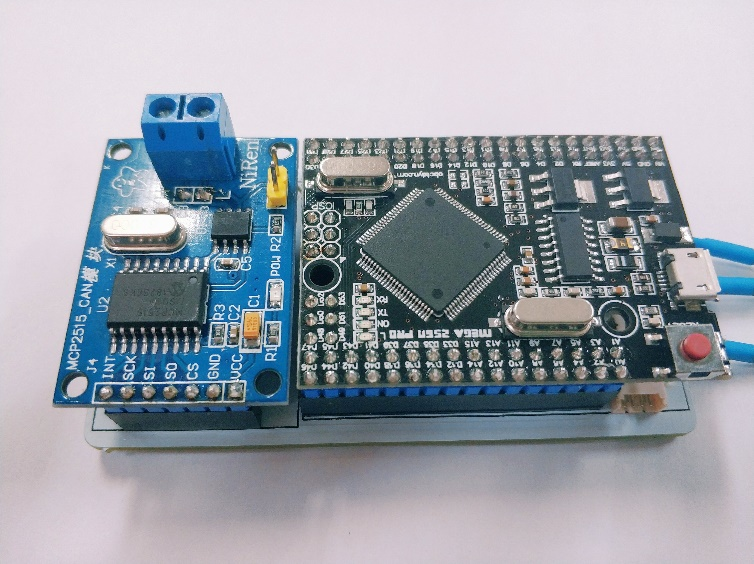
\includegraphics[width=7cm]{fig/f40.jpg}}\quad
    \label{fig:sub2}{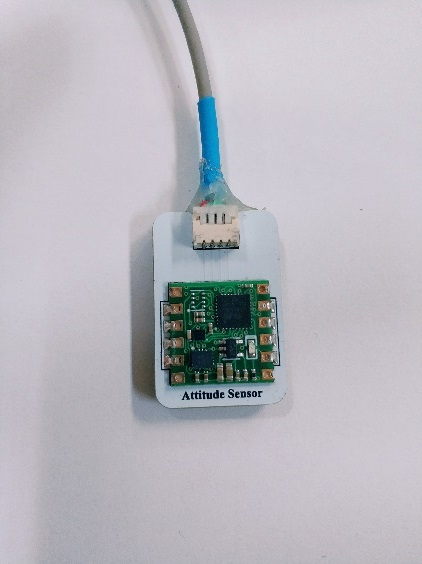
\includegraphics[width=4cm]{fig/f41.jpg}}
    \caption{基于IMU的姿态采集系统}
    \label{fig:subfigss}
\end{figure}

\begin{figure}[!h]
    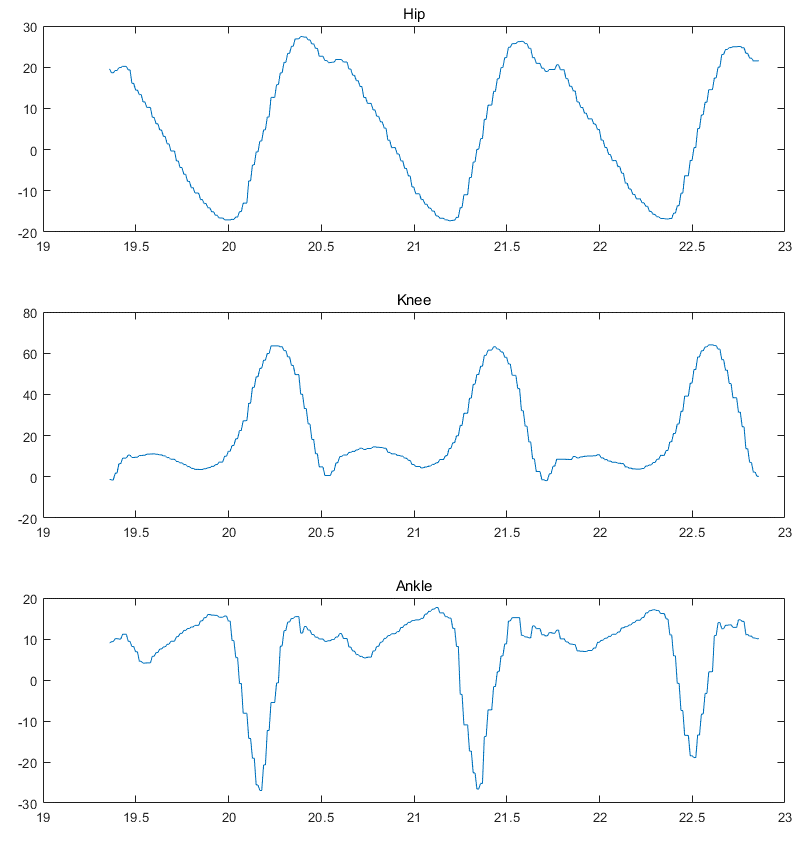
\includegraphics[width=13.5cm]{fig/f39.png}
    \caption{姿态采集系统得到的关节角度曲线}
    \label{fig:mark}
\end{figure}

为了测量人体的运动学数据,本文设计基于IMU的姿态测量系统,如图2.13所示,左图所示的为单个IMU模块,它可以被安装在身体的各个部分;右图为是数据采集与处理模块,它通过I2C总线连接三个IMU模块,通过Kalman滤波解算三个模块的姿态角度,之后将姿态角转换为人体的关节角度,并通过CAN总线发送给MicroLabBox。通过本文设计的姿态采集系统得到的关节角度曲线如图2.14所示。

\section{肌电信号采集与处理}
\subsection{肌电信号原理}
\begin{figure}[htb]
    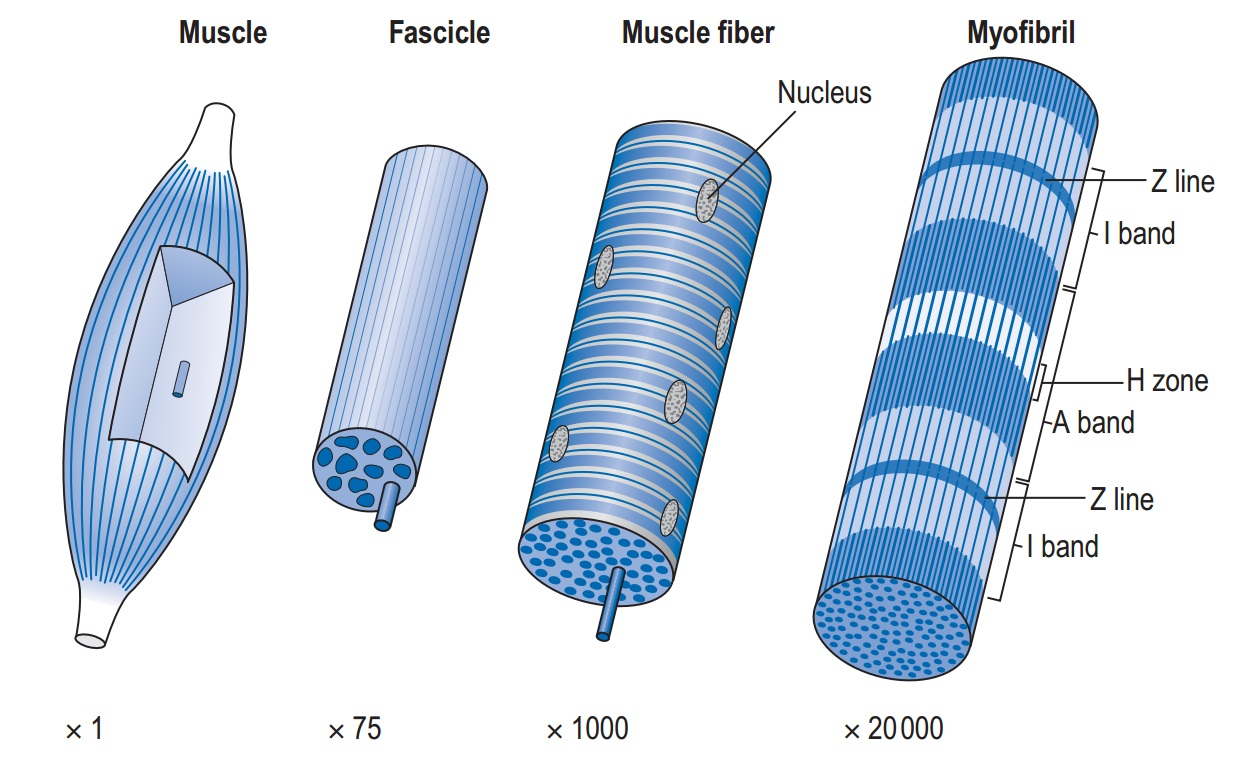
\includegraphics[width=14cm]{fig/f43.jpg}
    \caption{人体肌肉机结构示意图\cite{p44}}
    \label{fig:mark}
\end{figure}
人体有三种肌肉:平滑肌、心肌和骨骼肌,其中负责四肢的运动主要为骨骼肌。肌肉由数百个束组成,如图2.15,而每个束又由数百个肌纤维组成。肌纤维是肌肉组织的基本单位,其本身是由数百个肌原纤维组成的。这些肌原纤维具有典型的条纹状外观,条纹是由两种蛋白质——肌动蛋白和肌球蛋白——构成的有规则排列的丝状物,正是这些纤维通过桥的形成和破坏相互滑动导致肌肉收缩。在肌肉纤维的外面是毛细血管和运动神经的末端分支,它们在运动终端(神经肌肉接头)与肌肉纤维连接。平均一条运动神经会连接到大约150条肌纤维,神经元和它所支配的肌纤维的组合被称为运动单元。

\begin{figure}[htb]
    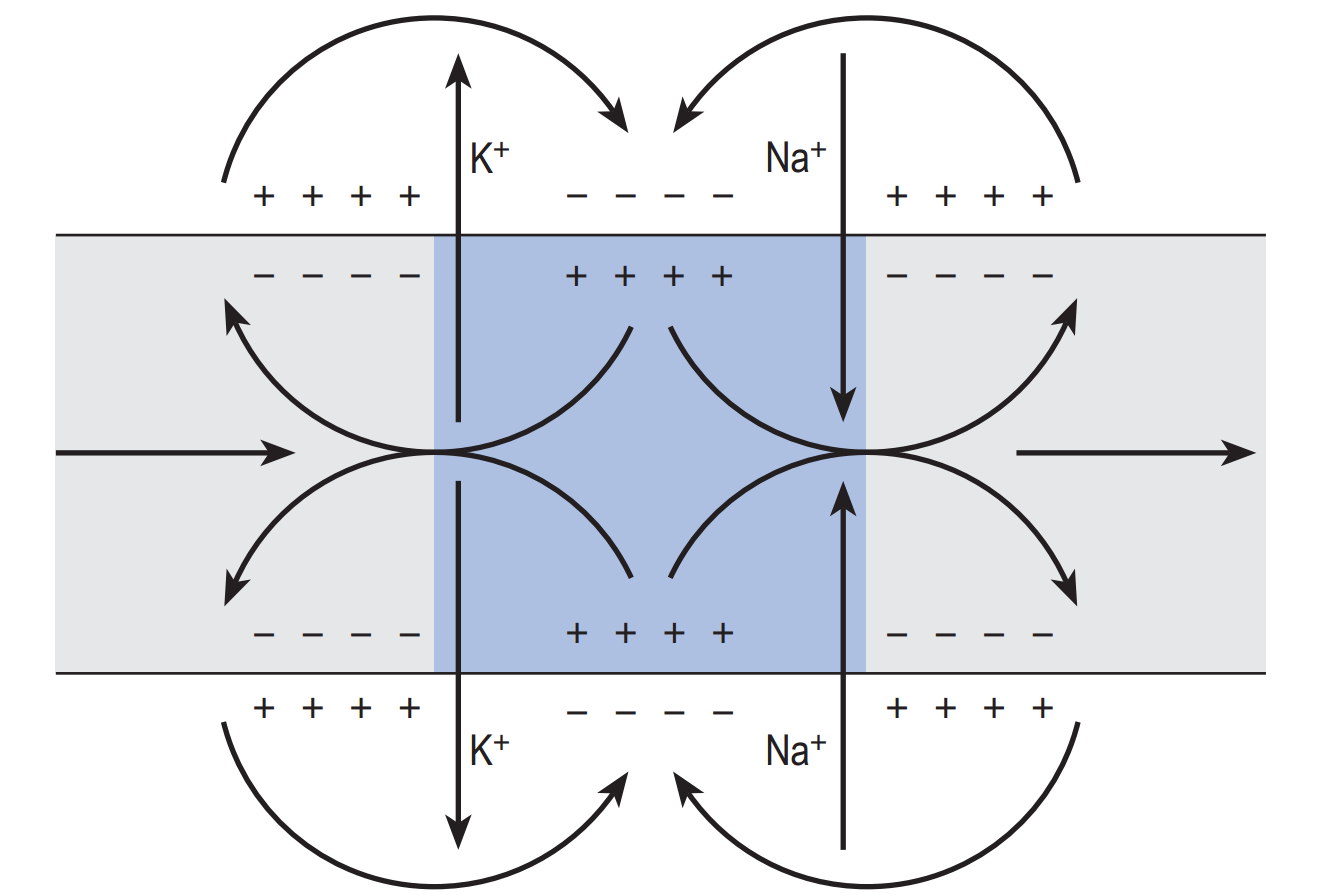
\includegraphics[width=10cm]{fig/f42.png}
    \caption{细胞动作电位示意图\cite{p44}}
    \label{fig:mark}
\end{figure}

当动作电位通过神经传递到运动终端时,会导致传递物质乙酰胆碱的释放,使肌纤维的细胞膜去极化。当这种肌肉动作电位在肌肉纤维中扩散时,它会导致钙离子的释放,从而触发肌肉收缩。肌动蛋白和肌球蛋白分子之间形成了桥梁,将它们拉在一起,这种张力维持了很短的一段时间,如果没有进一步的动作电位发生,就释放出来,钙离子被钙泵移除。如图2.16所示,肌肉动作电位的电活动可以检测出来,称为肌电图(EMG)。

EMG信号是众多运动单元动作电位在时间和空间上的叠加,根据具体测量方式又可分为针电极信号NEMG和表面肌电信号sEMG。表面肌电信号是浅层肌肉和神经电活动在皮肤表面的综合效应,能在一定程度上反映出神经肌肉的活动;相对于NEMG,SEMG在测量上具有非侵入性、操作简单等优点,因此广泛应用于临床医学、体育科学等领域。

\subsection{sEMG信号的采集与处理}
\begin{figure}[htb]
    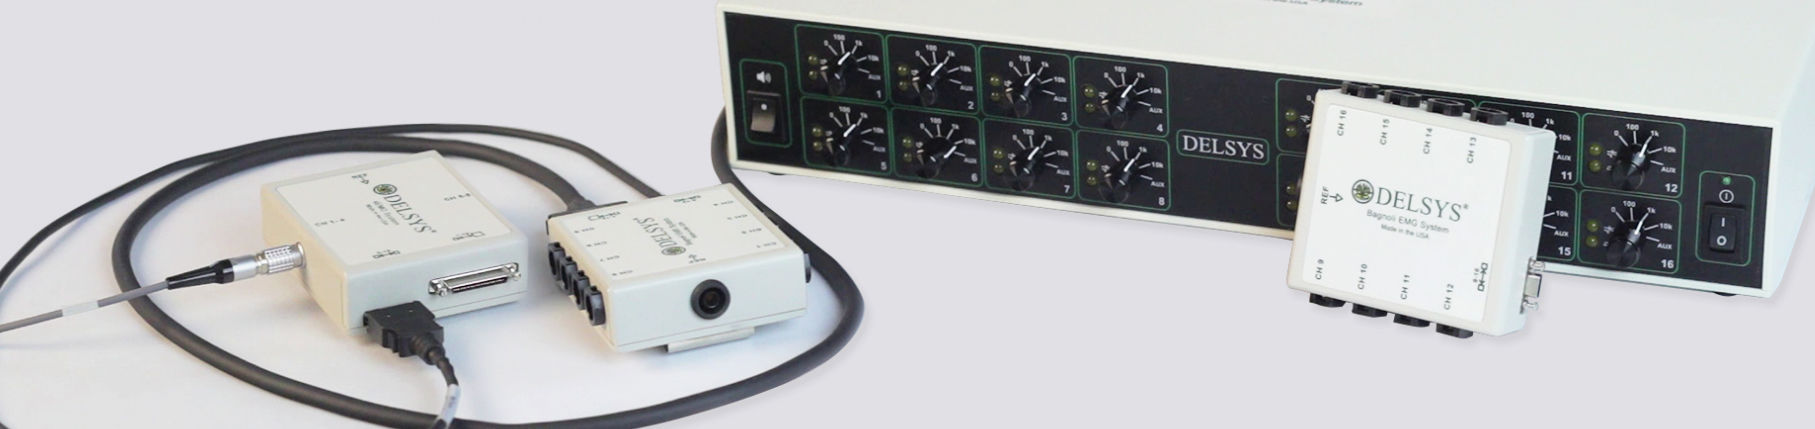
\includegraphics[width=16cm]{fig/f44.jpg}
    \caption{DELSYS 16通道EMG测量系统}
    \label{fig:mark}
\end{figure}
sEMG信号非常微弱,需要专用仪器进行采集。本文采用DELSYS公司生产的16通道EMG测量系统,可以实现16通道EMG数据的同时采集,采集的信号以模拟量形式连接到MicroLabBox的模拟量输入通道。以手臂的肱二头肌为例,采集的EMG如图2.18所示。

\begin{figure}[htb]
    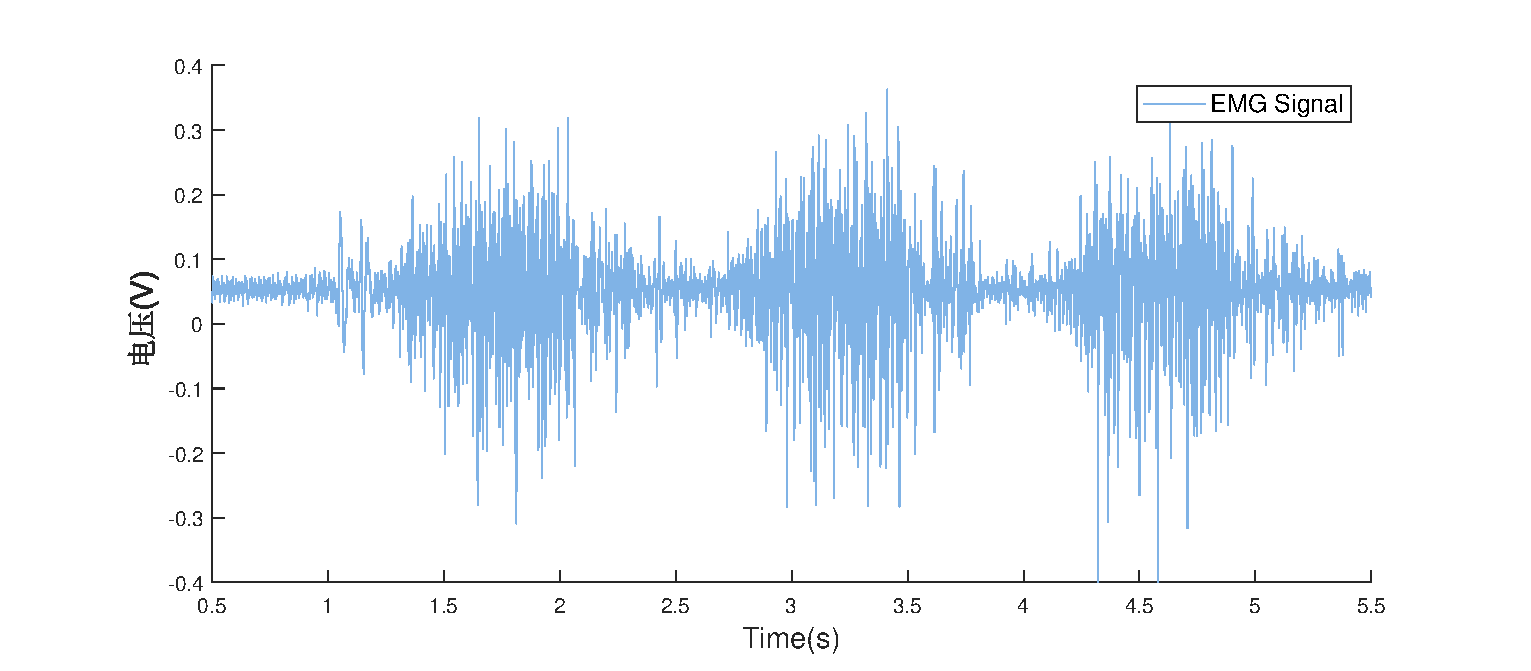
\includegraphics[width=17cm]{fig/f45.eps}
    \caption{肱二头肌收缩时的EMG信号}
    \label{fig:mark}
\end{figure}

\begin{figure}[htb]
    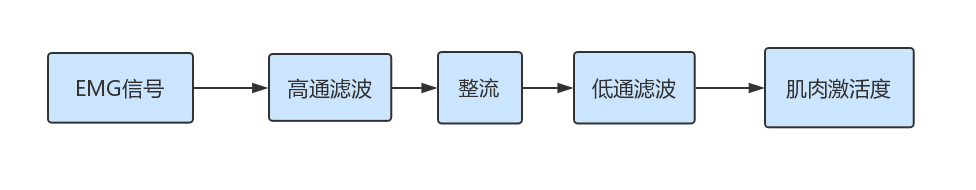
\includegraphics[width=16cm]{fig/f47.png}
    \caption{EMG信号处理流程}
    \label{fig:mark}
\end{figure}

\begin{figure}[!h]
    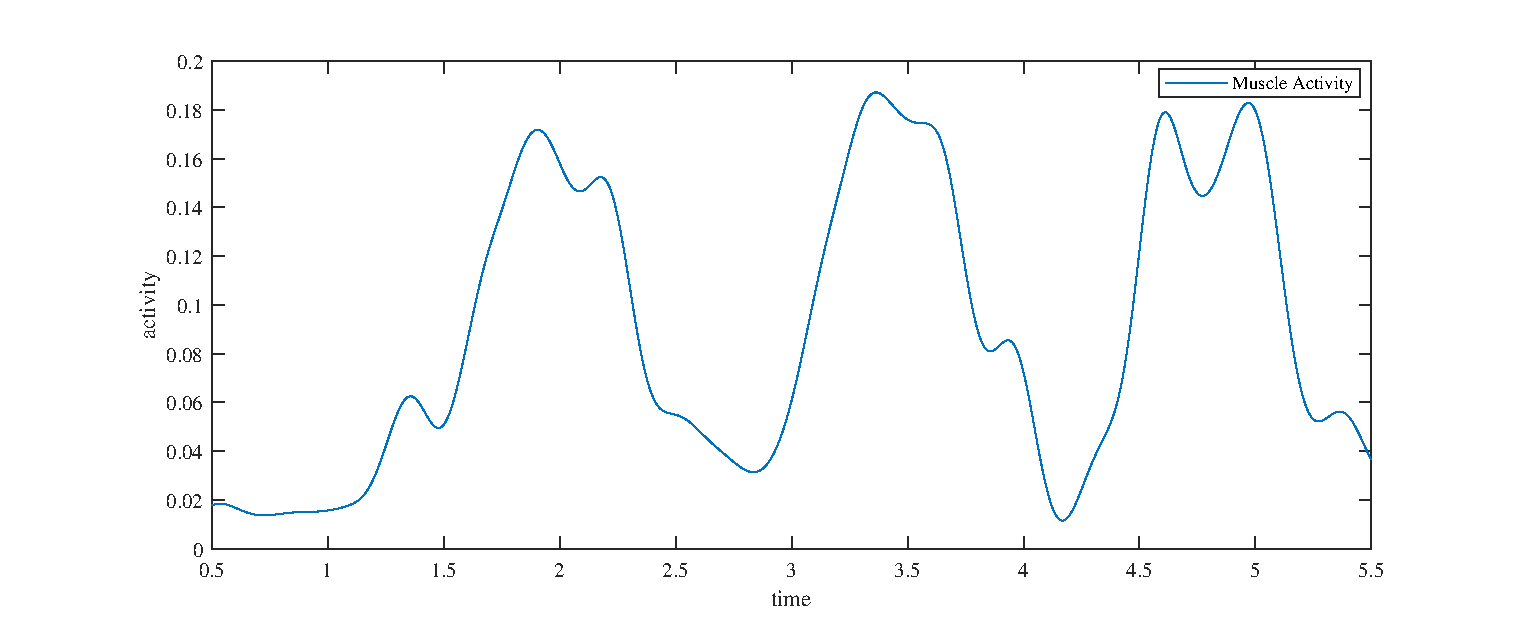
\includegraphics[width=17cm]{fig/f46.eps}
    \caption{肱二头肌收缩时的肌肉激活度曲线}
    \label{fig:mark}
\end{figure}

由于EMG信号是众多运动单元动作电位在时间和空间上的叠加,为典型的非平稳信号。生物学领域为从EMG信号中得到肌肉的激活的信息,较多的采用图2.19所示的方法对EMG进行滤波处理\cite{p45}。由于采集仪器和测量电路的影响,EMG信号中存在直流偏置,所以首先需要进行截止频率为25Hz高通滤波;之后对信号进行整流,再通过截止频率为4Hz的低通滤波器滤除高频分量,最终得到肌肉的激活信息。由图2.18 EMG信号滤波后的肌肉激活曲线如2.20所示。

\section{本章小结}

本章针对所研究的踝关节式外骨骼搭建了一套传感系统,搭建外骨骼力矩应变测量电路,使用足底开关检测人体的步态周期,设计了基于IMU的人体姿态数据采集系统,实现了基于EMG信号的肌肉激活度检测。除了上述部分外,该传感系统还包括测量电机角度的编码器、人体代谢数据的心肺呼吸仪和足底压力鞋垫等,但与本文后续内无密切关系,故不再加以赘述。